
\chapter{Materiais e Métodos}
\label{metodologia}
Este capítulo descreve os componentes do sistema proposto na \autoref{objetivos}.

\section{Arquitetura geral do sistema}
O sistema proposto para medir o tráfego de pessoas dentro de uma determinada zona a partir de sinais Wi-Fi é baseado no esquema da \autoref{esquema-geral} que será explicado pelos itens a seguir.

\begin{figure}[!h]
  \caption{\label{esquema-geral}Arquitetura geral do sistema}
  \begin{center}
    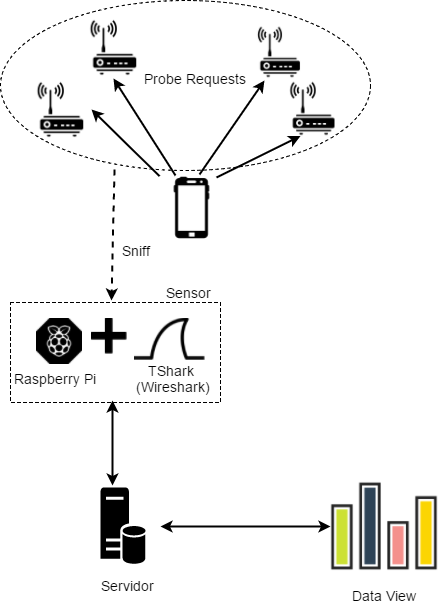
\includegraphics[width=0.50\textwidth]{img/esquema_geral.png}
  \end{center}
  \legend{Fonte: Elaborada pelas autoras.}
\end{figure}

\section{Detalhamento de processos}
O esquema da \autoref{esquema-geral} expõe de maneira mais abstrata o funcionamento do sistema de medição de tráfego. Já o diagrama de fluxo da \autoref{diagrama-fluxo} apresenta os processos, entidades externas e repositórios de armazenamento que compõe o sistema.

\begin{figure}[!h]
  \caption{\label{diagrama-fluxo}Processos e entidades do sistema}
  \begin{center}
    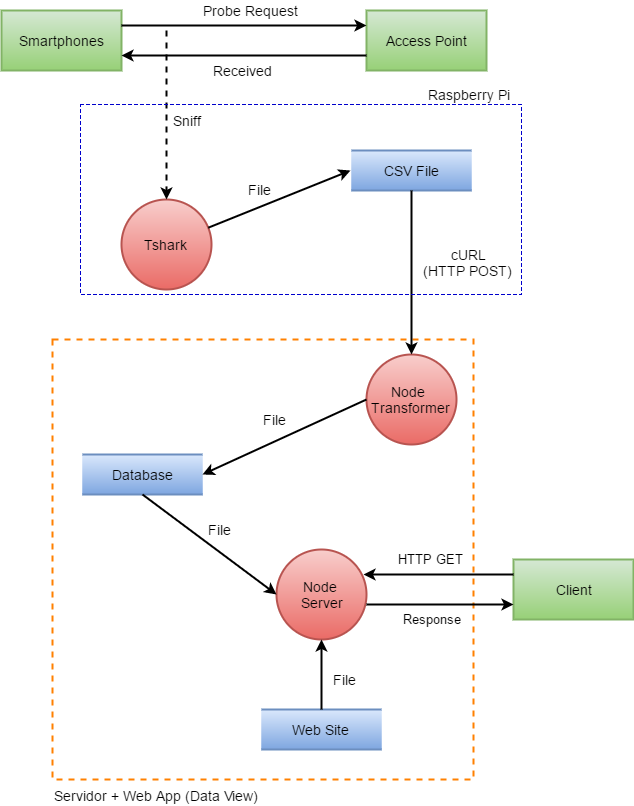
\includegraphics[width=0.70\textwidth]{img/diagrama_fluxo.png}
  \end{center}
  \legend{Fonte: Elaborada pelas autoras.}
\end{figure}

\section{Dispositivo Móvel e \emph{Probe Request}}
\label{smartphone-probe}
Para encontrar redes a que possa se conectar, um dispositivo móvel emite de tempos em tempos (depende da fabricante) pacotes do tipo \emph{probe request} para os APs próximos \cite{Meraki}. Todos os APs que receberem, responderão ao dispositivo (\emph{probe response} ou \emph{received}), então o aparelho descobrirá as redes ao redor disponíveis para conexão.

\section{Sensor}
O sensor é responsável pela detecção de aparelhos e envio de dados ao servidor.

\subsection{Raspberry Pi}
Para a detecção de dispositivos móveis um Raspberry Pi Model 3 B juntamente com um adaptador Wi-Fi são utilizados. O Raspberry foi escolhido,
pois oferece interface amigável de programação (Kali Linux); possui poder de processamento para receber os milhares de pacotes, pré-processá-los
e enviar para o servidor; possui entrada USB pode receber uma antena Wi-Fi e seu tamanho pequeno \cite{rpi2017}.

Outras opções foram consideradas por serem baratas, acessíveis e terem documentação aberta. Foi o caso do ESP8266 que possui um tamanho extremamente
reduzido e possui o custo médio de R\$15,00 \cite{Embarcados2015}, mas seu uso para este trabalho fica impossibilitado. Isso
ocorre, pois essa tecnologia não consegue ser habilitada para o modo monitor da interface de rede \cite{Puhl2016} \cite{Ferreira2016}.

Uma antena Wi-Fi (Ralink MT7601U) foi equipada no Raspberry para ampliar o alcance da captura já que o propósito do sistema é detecção em zonas que podem
apresentar esparcidade de indivíduos (espalhados) e já que ela pôde ser habilitada para o modo monitor (\autoref{modo-monitor}). A antena nativa
do Raspberry não conseguiu ser habilitada para o \emph{monitor mode}.

\subsection{Kali Linux}
O sistema operacional Kali Linux \cite{kali} foi escolhido para o Raspberry Pi, pois possui ampla documentação
para uso em projetos de redes, além de ferramentas, como suporte a drivers de interfaces de rede que possam
ser habilitadas para o modo monitor, foi o caso do Ralink MT7601U.

\subsection{Tshark}
O protocolo Tshark é uma versão de terminal do protocolo
analisador de rede Wireshark \cite{Wireshark2017} \cite{Wireshark2017a}. Ele é utilizado para analisar e filtrar (\emph{sniff}) e converter os dados dos pacotes capturados pelo sensor em arquivo formato CSV. Esse protocolo foi escolhido, pois permite realizar o estudo da rede a partir do recebimento de pacotes e seus campos, além possuir ampla documentação, maturidade e exemplos por ser uma tecnologia aberta.

\section{Servidor}
O servidor que servirá o Web App será baseado em Node.js. Ele possui duas partes principais que serão apresentadas a seguir.

\subsection{Node Transformer}
\label{node-transformer}
Após converter os dados do pacotes recebidos para um arquivo formato .CSV, o Raspberry Pi dá um cURL POST (HTTP POST através do terminal) de tempos em tempos para enviar o arquivo .CSV daquela sessão ao servidor. No servidor, o módulo node transformer particionará o arquivo (segundo alguns campos) em outros arquivos .JSON que serão salvos no banco de dados.

\subsection{Node Server}
 A partir dos arquivos .JSON citados no item anterior e um Web Site base (HTML, CSS, Javascript), o módulo Node Server responde (Response) à requisição do cliente (HTTP GET) e apresenta-o aos dados capturados.

\section{Data View}
O Data View é a parte do Web App responsável por apresentar os dados capturados de maneira clara e legível. Para isso, a biblioteca D3.js \cite{D32017} será utilizada para a plotagem de gráficos a partir dos arquivos .JSON.

\section{Protótipo}
Como apresentação parcial e prova de funcionamento dos componentes anteriores, o protótipo desenvolvido é baseado no sensor.
Trata-se de um Raspberry Pi equipado com um adaptador Wi-Fi que consegue capturar, analisar e exportar os pacotes
\emph{probe request} para um arquivo que será enviado ao servidor. Essa etapa é garantida pelo protocolo de análise de rede
Tshark.

Os comandos do Tshark que capturam os pacotes provenientes dos dispositivos móveis são realizados através de um servidor local
feito em Node.js, como mostra o código presente na \autoref{prototipo-app}.

\begin{figure}[!h]
  \caption{\label{prototipo-app}Protótipo do sistema}
  \begin{center}
    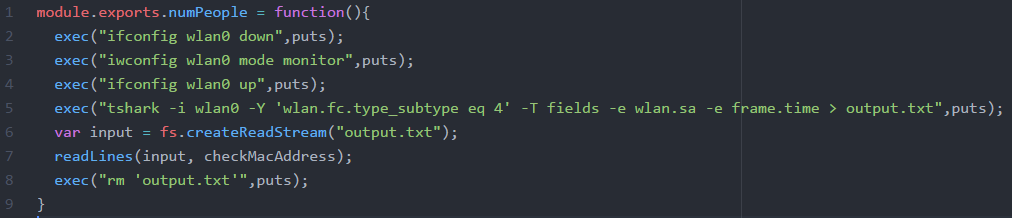
\includegraphics[width=1.0\textwidth]{img/prototipo-app.png}
  \end{center}
  \legend{Fonte: Elaborada pelas autoras.}
\end{figure}

A \autoref{prototipo-app} apresenta o código de um módulo Node.js que assemelha-se com a função que será desempenha
pelo Node Transformer (\autoref{node-transformer}). Esse módulo é chamado no servidor. As linhas que possuem o comando ``exec'' executam comandos diretamente
no terminal do sistema operaciomal. Nas linhas 2-4, habilita-se o adaptador de rede para o modo monitor. Na linha 5,
o comando Tshark rodado representa:

\begin{itemize}
  \item \textbf{wlan0}: interface de rede que indica a antena Wifi;
  \item \textbf{wlan.fc.type\_subtype eq 4}: indica que só pacotes \emph{probe request} devem ser capturados;
  \item \textbf{wlan.sa}: representa o \emph{source address} ou endereço MAC do dispositivo que enviou o pacote;
  \item \textbf{frame.time}: representa a hora, dia e ano em que o pacote foi capturado.
\end{itemize}

Em seguida no código, o arquivo exportado pelo Tshark é lido através de um \emph{stream}. A função ``readLines()''
na linha 7, lê o arquivo linha por linha, identificando os endereços MAC diferentes e adicionando-os a uma lista.
Então, nessa própria função é mostrado no terminal (``console.log(list)''), quantas pessoas foram contadas, ou em outros termos,
quantos dispositivos diferentes foram detectados. Na \autoref{arquivo-pacotes}, mostra-se o arquivo com os pacotes
capturados. Na \autoref{exec-bash} apresenta-se o que a execução da aplicação feita gerou, no caso, detectou
4 pessoas nas proximidades.

\begin{figure}[!h]
  \caption{\label{arquivo-pacotes}Arquivo com pacotes capturados}
  \begin{center}
    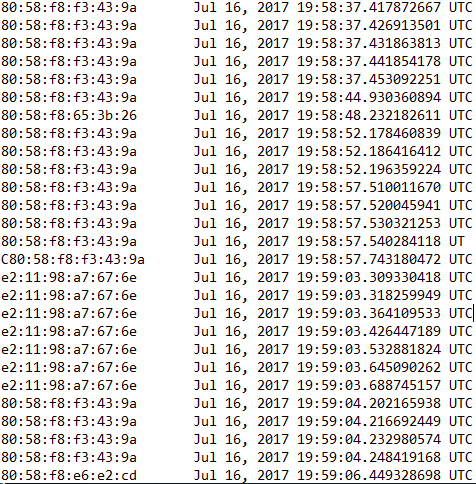
\includegraphics[width=0.70\textwidth]{img/packets.png}
  \end{center}
  \legend{Fonte: Elaborada pelas autoras.}
\end{figure}

\begin{figure}[!h]
  \caption{\label{exec-bash}Resultado da execução da aplicação}
  \begin{center}
    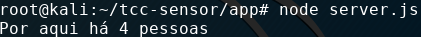
\includegraphics[width=1.0\textwidth]{img/bash.png}
  \end{center}
  \legend{Fonte: Elaborada pelas autoras.}
\end{figure}

\section{Testes e validação do projeto}
Para a validação do sistema proposto serão realizados testes unitários, de integração e
validação. Os testes unitários e de integração do sistema resumem-se em:

\begin{itemize}
  \item a detecção dos dispositivos móveis;
  \item comunicação entre Raspberry Pi e servidor;
  \item comunicação servidor e interface;
  \item processamento de dados capturados em dados desejados;
  \item determinar se sistema consegue contar pessoas.
\end{itemize}

Já os testes de validação são resumidos em determinar se o sistema consegue ou
não determinar a contagem e o tráfego de pessoas. Para tanto, serão feitos testes em
ambientes controlados e não controlados. Os controlados são
aquelas zonas em que sabe-se o número de pessoas, e então confere-se com o resultante da
detecção. Nos ambientes não-controlados, o tráfego de pessoas será testado.
A taxa de confiabilidade no sistema será baseada no desvio padrão dos testes
realizados em ambiente controlados.
O sistema final vai ser considerado aplicável ou não caso o desvio
padrão determinado fique dentro
dos limites.

Inicialmente, visa-se desenvolver os primeiros testes em ambiente
controlado, numa área pequena e com poucos dispositivos móveis, para verificar o
comportamento do sistema desenvolvido na medição do tráfego. Após testes
iniciais, pretende-se encontrar uma organização parceira que esteja dentro das
especificações necessárias e deseje conhecer melhor seu público alvo, cedendo
seu espaço e sua rede para alguns procedimentos e testes com a aplicação proposta
 - nessa etapa, o projeto busca verificar o desempenho do
sistema em ambiente real, com maior quantidade de dispositivos móveis.

\section{Análise de Riscos}
Considerando as premissas dos tópicos anteriores, há alguns itens e áreas que podem sofrer desvios ao longo do trabalho. Estes itens e seus planos
de contingência respectivamente são:

\begin{itemize}
  \item Falha da detecção de dispositivos (precisão): serão feitas duas formas de detecção através do protocolo Tshark, as duas garantem que os dados
  de uma e outra são verídicos, caso uma falhe há a outra para detectar os aparelhos móveis;
  \item Processamento no servidor é complexa: caso o desenvolvimento do processamento de dados no servidor seja muito complexa e considerando
  que trabalharemos com estatísticas, optar por uma \emph{cloud} seria uma opção;
  \item Raspberry Pi perder a conexão com a rede para mandar dados ao servidor: um backup dos dados será feito no aparelho, e então quando
  a conexão retornar, esses serão enviado ao servidor. Também há a possibilidade do uso de um Modem 3G para garantir o envio.
\end{itemize}
